\documentclass[12pt]{beamer}
\setbeamertemplate{navigation symbols}{}
\usetheme{Copenhagen}
\usepackage{listings}
\usepackage{xcolor}
\usepackage{graphicx}
\usepackage{hyperref}
\graphicspath{ {imagenes/} }

\definecolor{codegreen}{rgb}{0,0.6,0}
\definecolor{codegray}{rgb}{0.5,0.5,0.5}
\definecolor{codepurple}{rgb}{0.58,0,0.82}
\definecolor{backcolour}{rgb}{0.95,0.95,0.92}

\lstdefinestyle{mystyle}{
    language=c++,
    backgroundcolor=\color{backcolour},   
    commentstyle=\color{codegreen},
    keywordstyle=\color{magenta},
    numberstyle=\tiny\color{codegray},
    stringstyle=\color{codepurple},
    basicstyle=\ttfamily\footnotesize,
    breakatwhitespace=false,         
    breaklines=true,                 
    captionpos=b,                    
    keepspaces=true,                 
    numbers=left,                    
    numbersep=5pt,                  
    showspaces=false,                
    showstringspaces=false,
    showtabs=false,                  
    tabsize=2
}

\lstset{style=mystyle}

\title{Arreglos en C++}
\subtitle{Conceptos básicos}
\author{Tomás Peiretti}
\date{}

\begin{document}

\maketitle

\begin{frame}{¿Qué es un arreglo (array)?}
    Un arreglo es una \alert{serie de elementos de un mismo tipo} almacenados en posiciones contiguas de memoria que pueden ser referenciados individualmente a través de un índice.

    \medskip

    Por ejemplo, un arreglo llamado \alert{arr} que contiene 5 valores de tipo \alert{int} puede representarse de la siguiente manera:

    \medskip
    \begin{columns}
        \column{0.7\textwidth}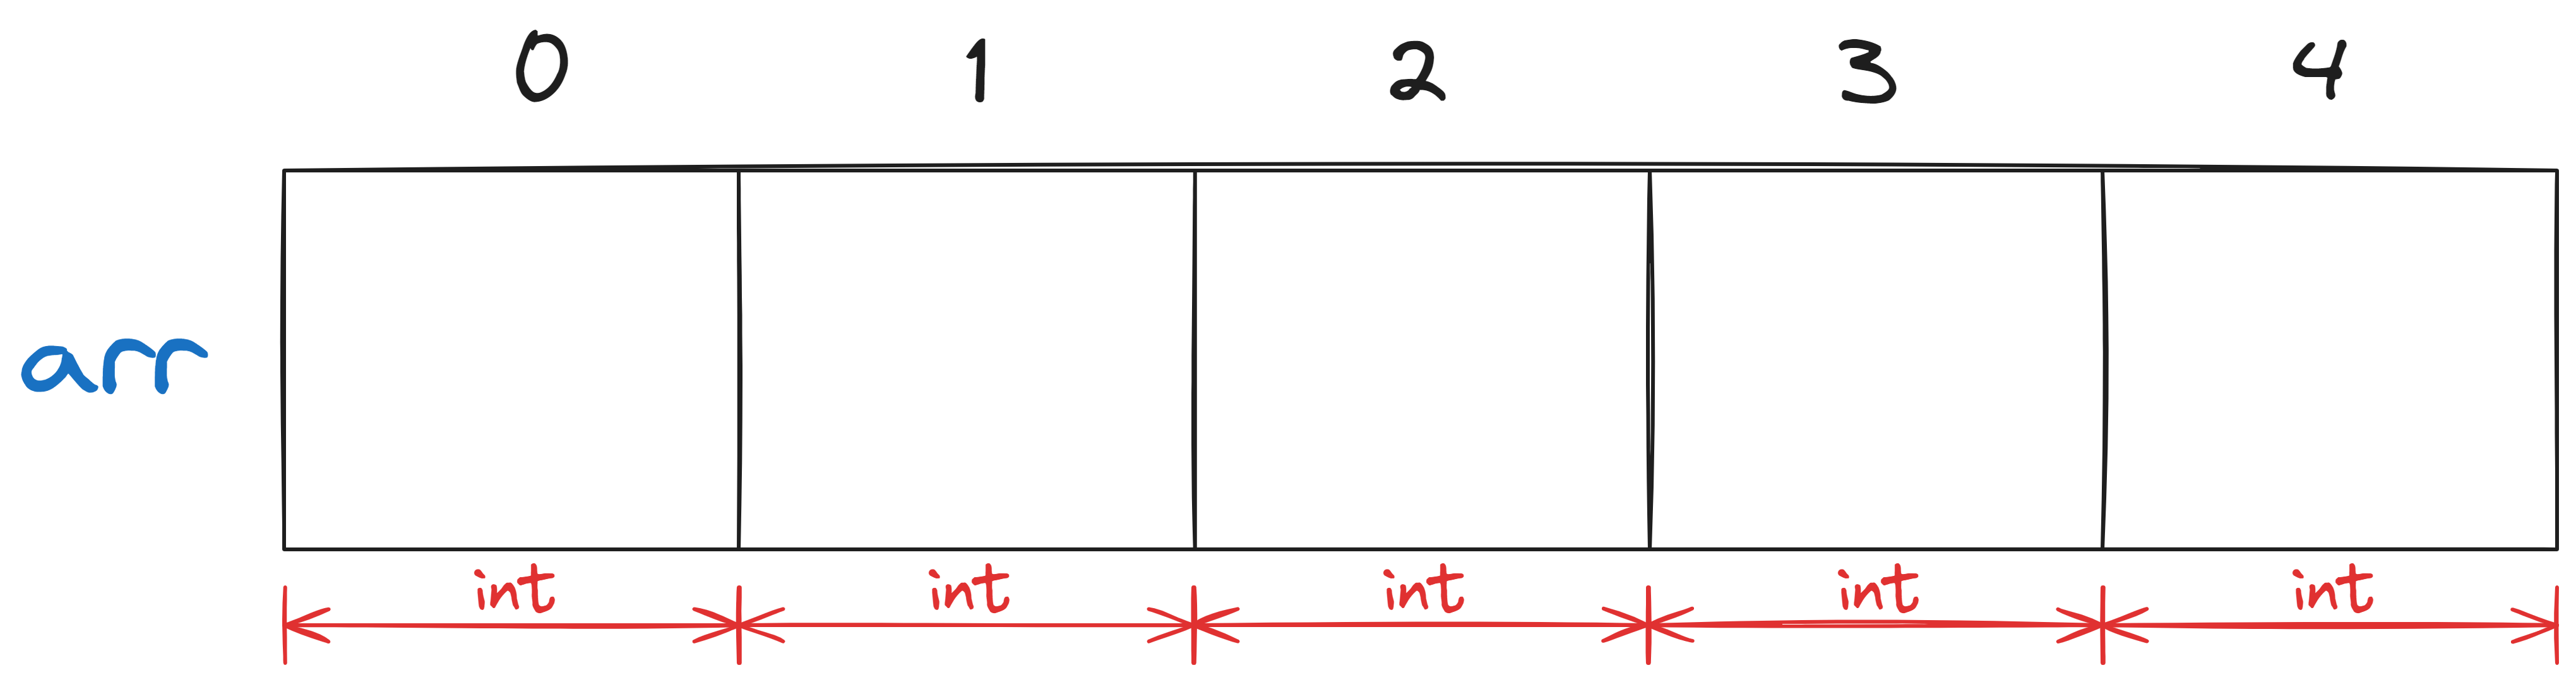
\includegraphics[width=\textwidth]{array1.png}
        \column{0.3\textwidth}
\includegraphics[width=\textwidth]{meme.jpg}
    \end{columns}
\end{frame}

\begin{frame}[fragile]{¿Qué es un arreglo (array)?}
    Al igual que las variables, un arreglo debe ser declarado antes de ser utilizado:
    \begin{center}
        \alert{tipo} nombre[tamaño];
    \end{center}

    Donde, el número de elementos (tamaño) del arreglo debe ser una expresión constante
    \begin{itemize}
        \item Puede utilizarse una constante literal (10, 200, 1573, etc), ó
        \item Puede utilizarse una constante global
    \end{itemize}
\begin{lstlisting}
#define tam 200
int main() {
    int arr1[10]; // constante literal
    int arr2[tam]; // constante global
    return 0;
}
\end{lstlisting}
\end{frame}

\begin{frame}[fragile]{Acceder a un elemento}
    Para acceder a un elemento del arreglo se utiliza la sintaxis \alert{nombre[indice]}. Ejemplos: \\
\begin{lstlisting}
int main() {
    char arreglo[100];
    // imprimir el elemento que se encuentra en el indice 43
    cout << arreglo[43] << endl;
    // guardar en el 3ra posicion el caracter X
    arreglo[2] = 'X';
    // imprimir los primeros 10 elementos
    for (int i=0; i<10; i++)
        cout << arreglo[i] << endl;
    
    return 0;
}
\end{lstlisting}
\end{frame}

\begin{frame}[fragile]{Inicializar un arreglo}
    \begin{columns}
        \column{0.5\textwidth}Por defecto, los arreglos de alcance local se encuentran sin inicializar, por lo que contienen valores "basura" almacenados en las diferentes posiciones.
        \column{0.5\textwidth}\begin{lstlisting}[basicstyle=\tiny]
int main() {
    int arr0[5]; // sin inicializar
    int arr1[] = {1, 23, -2, 4, 1};
    int arr2[5] = {10, 15, 2};
    int arr3[5] = {};
    int arr4[] {5, 14, 25};

    int arr5[5];
    for(int i=0; i<5; i++)
        arr5[i]=7;

    return 0;
}
\end{lstlisting}
        \end{columns}
        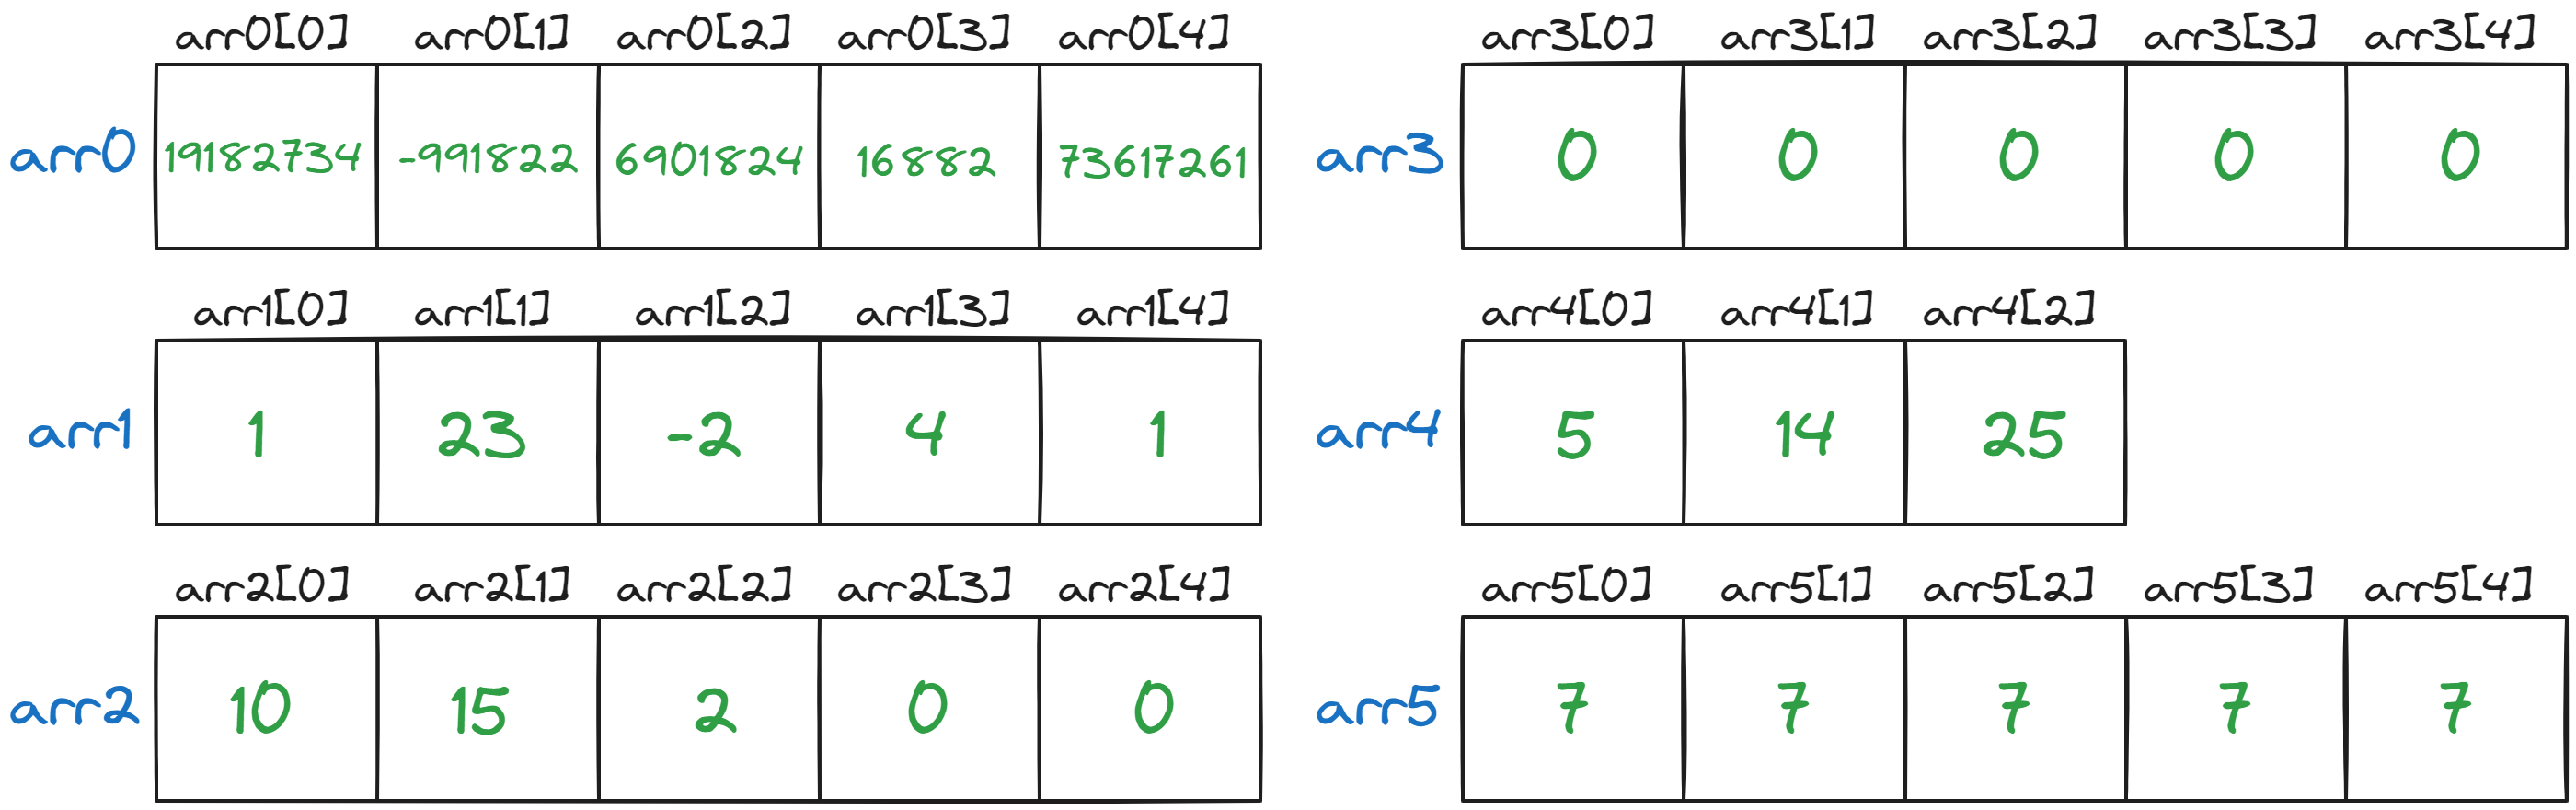
\includegraphics[width=\textwidth]{arrays.png}
\end{frame}

\begin{frame}[fragile]{Tamaño físico vs tamaño lógico}
    El \alert{tamaño físico} de un arreglo es el tamaño que se define al momento de declarar un arreglo. Es la cantidad maxima de elementos/posiciones que se pueden utilizar.
    
    \medskip
    
    En cambio, el \alert{tamaño lógico} refiere a la cantidad de posiciones/elementos que se estan utilizando y siempre \alert{debe ser menor o igual al tamaño físico}.

\begin{lstlisting}[]
// Ejemplo: arreglo con TF=10 y TL=5
int main() {
    int arreglo[10] = {1, 2, 3, 4, 5};
    for (int i=0; i<5; i++)
        cout << arreglo[i] << endl;
    return 0;
}
\end{lstlisting}
    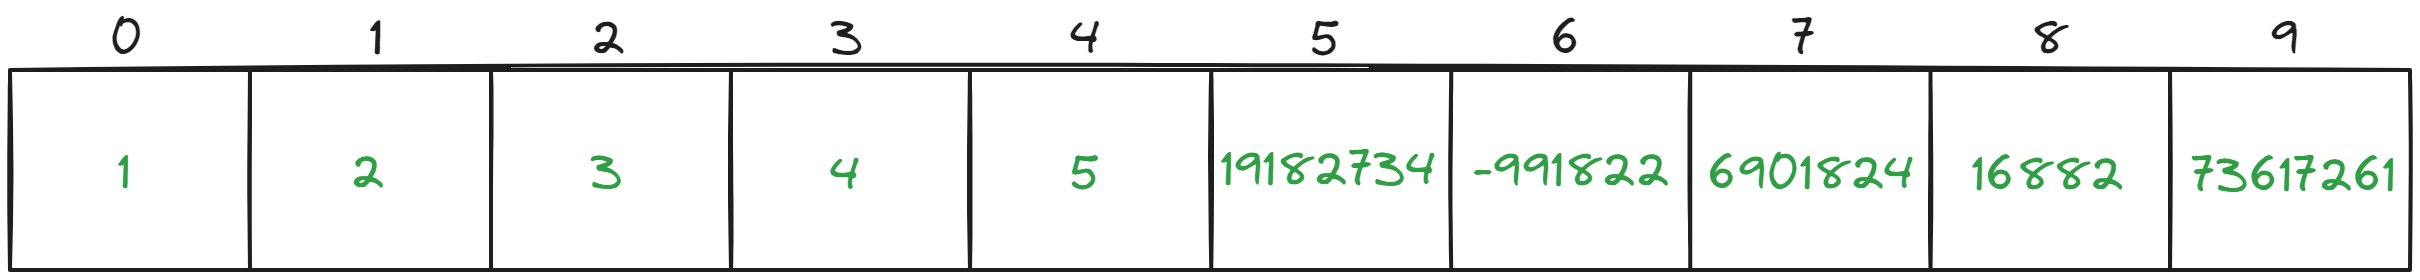
\includegraphics[width=\textwidth]{tamlogico.png}
\end{frame}

\begin{frame}{Operaciones con arreglos}
    ¿Qué operaciones debemos saber realizar con los arreglos para aprobar AEDD?
    \begin{itemize}
        \item Recorrer (de izq a derecha, en un rango, de der a izq, etc)
        \item Buscar un elemento
        \item Unir dos arreglos
        \item Invertir un arreglo
        \item Eliminar/agregar un elemento
        \item Ordenar (BubbleSort, MergeSort, SelectionSort, InsertionSort)
    \end{itemize}
\end{frame}

\begin{frame}{Ejercicios}
    \begin{itemize}
        \item \href{https://judge.beecrowd.com/es/problems/view/1173}{Beecrowd 1173}
        \item \href{https://judge.beecrowd.com/es/problems/view/1174}{Beecrowd 1174}
        \item \href{https://judge.beecrowd.com/es/problems/view/1177}{Beecrowd 1177}
        \item \href{https://judge.beecrowd.com/es/problems/view/1178}{Beecrowd 1178}
        \item \href{https://judge.beecrowd.com/es/problems/view/1180}{Beecrowd 1180}
        \item \href{https://codeforces.com/group/yg7WhsFsAp/contest/355494/problem/P25}{Codeforces ([GYM] 100 Easy Problems) P25}
        \item \href{https://judge.beecrowd.com/es/problems/view/1175}{Beecrowd 1175}
        \item \href{https://judge.beecrowd.com/es/problems/view/1171}{Beecrowd 1171}
        \item \href{https://judge.beecrowd.com/es/problems/view/1410}{Beecrowd 1410}
        \item \href{https://codeforces.com/group/yg7WhsFsAp/contest355490/problem/P02}{Codeforces ([GYM] 100 Easy Problems) P02}
    \end{itemize}
\end{frame}

\end{document}